\experiment{Binary Search Tree}{26/11/2023}

\section{Aim}
To implement a program for Binary Search Tree operations -  insert, delete, search.

\section{Algorithm}
 {\fontfamily{lmtt}\selectfont

  \subsection{Structure Definition}
  Create a structure \texttt{Node} with the following attributes:
  \begin{enumerate}[label=\arabic*:,left=0pt]
    \item Integer \texttt{data} to store the data of the node.
    \item Pointer to \texttt{Node} \texttt{left} to store the address of the left child.
    \item Pointer to \texttt{Node} \texttt{right} to store the address of the right child.
  \end{enumerate}

  \subsection{Insert Function}
  Create a function \texttt{insert(root, data)}:
  \begin{enumerate}[label=\arabic*:,left=0pt]
    \item \textbf{Start}
    \item Allocate memory for a new \texttt{Node} structure using \texttt{malloc}.
    \item Set \texttt{new->data} to \texttt{data}.
    \item Set \texttt{new->left} and \texttt{new->right} to \texttt{NULL}.
    \item If \texttt{root} is \texttt{NULL}, set \texttt{root} to \texttt{new} and return \texttt{root}.
    \item Create a \texttt{Node} pointer \texttt{ptr} and set it to \texttt{root}.
    \item Create a \texttt{Node} pointer \texttt{prev} and set it to \texttt{root}.
    \item Loop while \texttt{ptr} is not \texttt{NULL}:
          \begin{enumerate}[label=8.\arabic*:, start=1]
            \item Set \texttt{prev} to \texttt{ptr}.
            \item If \texttt{data > ptr->data}, set \texttt{ptr} to \texttt{ptr->right}.
            \item If \texttt{data < ptr->data}, set \texttt{ptr} to \texttt{ptr->left}.
            \item If \texttt{data == ptr->data}, print "Node already exists!" and return \texttt{root}.
          \end{enumerate}
    \item If \texttt{data > prev->data}, set \texttt{prev->right} to \texttt{new}.
    \item Otherwise, set \texttt{prev->left} to \texttt{new}.
    \item Return \texttt{root}.
    \item \textbf{Stop}
  \end{enumerate}

  \subsection{Inorder Successor Function}
  Create a function \texttt{inorderSuccessor(n)}:
  \begin{enumerate}[label=\arabic*:,left=0pt]
    \item \textbf{Start}
    \item Create \texttt{Node} pointers \texttt{current} and \texttt{prev}.
    \item If \texttt{n->right == NULL} or \texttt{n->left == NULL}, print "Node is empty to find null pointer!" and \newline return \texttt{n}.
    \item Set \texttt{current} and \texttt{prev} to \texttt{n}.
    \item Set \texttt{current} to \texttt{current->right}.
    \item Loop while \texttt{current != NULL}:
          \begin{enumerate}[label=6.\arabic*:, start=1]
            \item Set \texttt{prev} to \texttt{current}.
            \item Set \texttt{current} to \texttt{current->left}.
          \end{enumerate}
    \item Return \texttt{prev}.
    \item \textbf{Stop}
  \end{enumerate}

  \subsection{Delete Function}
  Create a function \texttt{delete(root, key)}:
  \begin{enumerate}[label=\arabic*:,left=0pt]
    \item \textbf{Start}
    \item Create \texttt{Node} pointers \texttt{current} and \texttt{prev}.
    \item Loop while \texttt{current != NULL}:
          \begin{enumerate}[label=3.\arabic*:, start=1]
            \item Set \texttt{prev} to \texttt{current}.
            \item If \texttt{current->data == key}, check for cases:
                  \begin{enumerate}[label=3.2.\arabic*:, start=1]
                    \item If \texttt{current->left != NULL} and \texttt{current->right != NULL}:
                          \begin{enumerate}[label=3.2.1.\arabic*:, start=1]
                            \item Create \texttt{Node} pointer \texttt{successor} and set it to \texttt{inorderSuccessor(current)}.
                            \item Set \texttt{current->data} to \texttt{successor->data}.
                            \item Free \texttt{successor}.
                          \end{enumerate}
                    \item If \texttt{current->left == NULL} or \texttt{current->right == NULL}:
                          \begin{enumerate}[label=3.2.2.\arabic*:, start=1]
                            \item Create \texttt{Node} pointer \texttt{child} and set it to \texttt{current->left}.
                            \item If \texttt{current->right != NULL}, set \texttt{child} to \texttt{current->right}.
                            \item If \texttt{current == root}, set \texttt{root} to \texttt{child}.
                            \item If \texttt{prev->left == current}, set \texttt{prev->left} to \texttt{child}.
                            \item Otherwise, set \texttt{prev->right} to \texttt{child}.
                            \item Free \texttt{current}.
                          \end{enumerate}
                    \item Print "Item deleted successfully!".
                    \item Return \texttt{root}.
                  \end{enumerate}
            \item If \texttt{current->data < key}, set \texttt{current} to \texttt{current->right}.
            \item Otherwise, set \texttt{current} to \texttt{current->left}.
          \end{enumerate}
    \item Print "Item not found!".
    \item Return \texttt{root}.
    \item \textbf{Stop}
  \end{enumerate}

  \subsection{Search Function}
  Create a function \texttt{search(root, key)}:
  \begin{enumerate}[label=\arabic*:,left=0pt]
    \item \textbf{Start}
    \item Create a \texttt{Node} pointer \texttt{current} and set it to \texttt{root}.
    \item Print "Searching - ".
    \item Loop while \texttt{current != NULL}:
          \begin{enumerate}[label=1.\arabic*:, start=1]
            \item Print \texttt{current->data}.
            \item If \texttt{current->data == key}, print "Item found!" and return.
            \item If \texttt{current->data < key}, set \texttt{current} to \texttt{current->right}.
            \item Otherwise, set \texttt{current} to \texttt{current->left}.
          \end{enumerate}
    \item Print "Item not found!".
    \item \textbf{Stop}
  \end{enumerate}

  \subsection{Main Function}
  \begin{enumerate}[label=\arabic*:,left=0pt]
    \item \textbf{Start}
    \item Set integer \texttt{ch}.
    \item Print menu options.
    \item Loop while \texttt{ch != 4}:
          \begin{enumerate}[label=4.\arabic*:, start=1]
            \item Print "Choice: ".
            \item Take user input for \texttt{ch}.
            \item If \texttt{ch == 1}, call \texttt{display(root)}.
            \item If \texttt{ch == 2}:
                  \begin{enumerate}[label=4.4.\arabic*:, start=1]
                    \item Set integer \texttt{x}.
                    \item Print "Enter the data: ".
                    \item Take user input for \texttt{x}.
                    \item Call \texttt{insert(root, x)} and assign the result to \texttt{root}.
                  \end{enumerate}
            \item If \texttt{ch == 3}:
                  \begin{enumerate}[label=4.5.\arabic*:, start=1]
                    \item Set integer \texttt{x}.
                    \item Print "Enter the key to delete: ".
                    \item Take user input for \texttt{x}.
                    \item Call \texttt{delete(root, x)} and assign the result to \texttt{root}.
                  \end{enumerate}
            \item If \texttt{ch != 4} and \texttt{ch} is not one of the above options, print "Invalid option!".
          \end{enumerate}
    \item \textbf{Stop}
  \end{enumerate}

 }

\section{C Program}
\begin{lstlisting}[label={list:c_program:binary_search_tree}]
#include <stdlib.h>
#include <stdio.h>

typedef struct Node
{
  int data;
  struct Node *left;
  struct Node *right;
} node;

// Binary Tree
node *insert(node *root, int data);
void search(node *root, int key);
node *delete(node *root, int key);

int main()
{
  node *root = NULL;

  int ch;
  printf("\n1)Insert Node\n2)Search Node\n3)Delete Node\n5)Exit");
  do
  {
    printf("\nChoice: ");
    scanf("%d", &ch);
    if (ch == 1)
    {
      int x;
      printf("\nEnter the data: ");
      scanf("%d", &x);
      root = insert(root, x);
    }
    else if (ch == 2)
    {
      int x;
      printf("\nEnter the key to search: ");
      scanf("%d", &x);
      search(root, x);
    }
    if (ch == 3)
    {
      int x;
      printf("\nEnter the key to delete: ");
      scanf("%d", &x);
      root = delete (root, x);
    }
  } while (ch != 4);
}

node *insert(node *root, int data)
{
  node *new = (node *)malloc(sizeof(node));
  new->data = data;
  new->left = NULL;
  new->right = NULL;
  if (root == NULL)
  {
    root = new;
    return root;
  }
  node *ptr = root;
  node *prev = root;
  while (ptr != NULL)
  {
    prev = ptr;
    if (data > ptr->data)
    {
      ptr = ptr->right;
    }
    else if (data < ptr->data)
    {
      ptr = ptr->left;
    }
    else
    {
      printf("\nNode already exist!!\n");
      return root;
    }
  }
  if (data > prev->data)
  {
    prev->right = new;
  }
  else
  {
    prev->left = new;
  }
  return root;
}

node *inorderSuccessor(node *n)
{
  node *current;
  node *prev;
  if (n->right == NULL || n->left == NULL)
  {
    printf("\nNode is empty to find null pointer!!\n");
    return n;
  }
  current = n;
  prev = n;
  current = current->right;
  while (current != NULL)
  {
    prev = current;
    current = current->left;
  }
  return prev;
}

node *delete(node *root, int key)
{
  node *current = root;
  node *prev = NULL;
  while (current != NULL)
  {
    if (current->data == key)
    {
      if (current->left != NULL && current->right != NULL)
      {
        node *successor = inorderSuccessor(current);
        // printf("\nInorder successor = %d", successor->data);
        current->data = successor->data;
        free(successor);
      }
      else
      {
        node *child = current->left;
        if (current->right != NULL)
        {
          child = current->right;
        }
        if (current == root)
        {
          root = child;
        }
        else if (prev->left == current)
        {
          prev->left = child;
        }
        else
        {
          prev->right = child;
        }
        free(current);
      }
      printf("\nItem deleted successfully!!\n");
      return root;
    }
    else if (current->data < key)
    {
      prev = current;
      current = current->right;
    }
    else
    {
      prev = current;
      current = current->left;
    }
  }
  printf("\nItem not found!!\n");
  return root;
}

void search(node *root, int key)
{
  node *current = root;
  printf("\nSearching - ");
  while (current != NULL)
  {
    printf(" %d ", current->data);
    if (current->data == key)
    {
      printf("\nItem found!\n");
      return;
    }
    else if (current->data < key)
    {
      current = current->right;
    }
    else
    {
      current = current->left;
    }
  }
  printf("\nItem not found!!\n");
}

\end{lstlisting}

\section{Output}
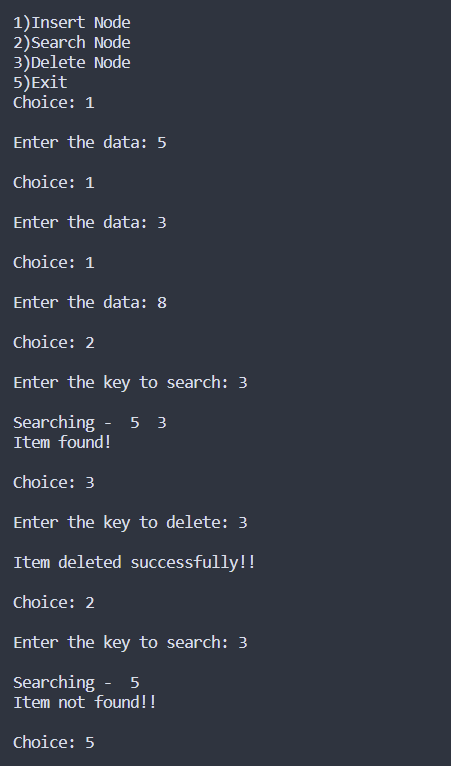
\includegraphics[]{Cycle_2/Outputs/BinarySearchTree.png}

\section{Result}
The Binary Search Tree operations were performed successfully. Output was verified.